\documentclass[conference]{IEEEtran}
\IEEEoverridecommandlockouts
% Template version as of 6/27/2024

\usepackage{cite}
\usepackage{amsmath,amssymb,amsfonts}
\usepackage{algorithmic}
\usepackage{graphicx}
\usepackage{textcomp}
\usepackage{xcolor}
\usepackage{booktabs}
\usepackage{multirow}
\usepackage{tikz}
\usetikzlibrary{shapes.geometric, arrows, positioning}

\def\BibTeX{{\rm B\kern-.05em{\sc i\kern-.025em b}\kern-.08em
    T\kern-.1667em\lower.7ex\hbox{E}\kern-.125emX}}

\begin{document}

\title{Multi-Agent LLM Orchestration for Claim Authentication via Semantic Codebase Vectorization}

\author{
\IEEEauthorblockN{M. Mounika}
\IEEEauthorblockA{\textit{Dept. of CSE (AI \& ML)} \\
\textit{B V Raju Institute of Technology}\\
Narsapur, Medak, Telangana, India \\
mounika.m@bvrit.ac.in}
\and
\IEEEauthorblockN{B. Lavanya}
\IEEEauthorblockA{\textit{Dept. of CSE (AI \& ML)} \\
\textit{B V Raju Institute of Technology}\\
Narsapur, Medak, Telangana, India \\
Lavanya.b@bvrit.ac.in}
\and
\IEEEauthorblockN{Abhinav Basam}
\IEEEauthorblockA{\textit{Dept. of CSE (AI \& ML)} \\
\textit{B V Raju Institute of Technology}\\
Narsapur, Medak, Telangana, India \\
24211A6609@bvrit.ac.in}
\and
\IEEEauthorblockN{G. Uday Kiran}
\IEEEauthorblockA{\textit{Dept. of CSE (AI \& ML)} \\
\textit{B V Raju Institute of Technology}\\
Narsapur, Medak, Telangana, India \\
udaykiran.goru@bvrit.ac.in}
\and
\IEEEauthorblockN{B. Priyanka}
\IEEEauthorblockA{\textit{Dept. of CSE (AI \& ML)} \\
\textit{B V Raju Institute of Technology}\\
Narsapur, Medak, Telangana, India \\
priyanka.b@bvrit.ac.in}
\and
\IEEEauthorblockN{B. VeeraSekhar}
\IEEEauthorblockA{\textit{Dept. of CSE (AI \& ML)} \\
\textit{B V Raju Institute of Technology}\\
Narsapur, Medak, Telangana, India \\
veerasekharreddy.b@bvrit.ac.in}
}

\maketitle

\begin{abstract}
Contemporary automated Applicant Tracking Systems (ATS) and modern resume screening platforms primarily rely on textual keyword matching or ungrounded generative summaries to evaluate applicants. Consequently, such systems remain vulnerable to keyword stuffing and inflated skill assertions without verifying whether candidates have practically implemented their claimed technical proficiencies in working source code. In this research paper, we introduce CodeAudit AI, an end-to-end multi-agent framework that autonomously authenticates technical skill claims on resumes against candidates' public open-source software repositories. The proposed architecture includes four phases: (1) a PDF Resume Extraction agent that extracts skill claims and repository handles from PDF resumes; (2) an Asynchronous Ingestion agent that retrieves and filters source code; (3) a Retrieval-Augmented Generation (RAG) indexing agent that generates 384-dimensional dense vector embeddings grounded in source code with multi-tenant isolation; and (4) a Large Language Model (LLM) Judge agent operating under rigorous Chain-of-Thought evaluation rubrics. Evaluated on a primary 30-case benchmark and an extended 150-instance cohort, CodeAudit AI achieves 93.3\% and 92.7\% accuracy, respectively, while maintaining 100.0\% precision (0.0\% false positive rate) across all evaluations and a 94.7\% F1-score, outperforming traditional baselines by up to 33.3 percentage points. Crucially, the system achieves zero false positives (100.0\% specificity), ensuring that unsupported claims are never erroneously validated. Comprehensive sensitivity analyses justify the 800-character chunk window, demonstrate deterministic stability (variance $\sigma^2 = 0.000$) at zero sampling temperature, and confirm practical end-to-end latency of 7.27 s per applicant at a cost of \$0.008 per audit.
\end{abstract}

\begin{IEEEkeywords}
Multi-Agent Systems, Retrieval-Augmented Generation, Resume Verification, Large Language Models, Technical Skill Validation, Code Retrieval, ChromaDB.
\end{IEEEkeywords}

%=============================================================================
\section{Introduction}
%=============================================================================

One of the central components of modern talent acquisition is automated resume screening \cite{sinha2021resumescreening, alamri2022nlp}. However, candidate resumes frequently exaggerate programming language skills and software framework proficiencies \cite{deshpande2023candidate}. Conventional recruitment systems assess candidate suitability by computing lexical overlap and semantic similarity between candidate resumes and job descriptions \cite{lo2025aihiring}. Because these tools rely exclusively on unverified self-reported text, they cannot determine whether a candidate has genuine practical software development experience.

This operational blindspot introduces critical risks into technical hiring. Candidates can exploit lexical matching mechanisms through keyword stuffing, inflating competency statements, or using generative AI assistance to tailor resumes \cite{brown2020gpt3}. While open-source collaboration platforms like GitHub provide verifiable public audit trails of software development activity \cite{kalliamvakou2014github, vasilescu2015developer}, manual repository inspection by technical recruiters is labor-intensive and unscalable for large applicant pools.

Existing automated recruitment systems present three primary limitations:
\begin{enumerate}
    \item \textbf{Absence of Empirical Evidence Grounding:} Classical ML screening models \cite{sinha2021resumescreening} and NLP ranking pipelines \cite{alamri2022nlp} evaluate self-reported textual claims without inspecting underlying source code implementations.
    \item \textbf{Vulnerability to Hallucinations:} Direct generative assessment of candidate claims without structured code retrieval frequently generates hallucinations and false positive approvals \cite{lewis2020rag}.
    \item \textbf{Monolithic Architectural Rigidity:} Monolithic single-prompt models struggle with disparate multi-step tasks such as document parsing, code ingestion, and structured adjudication.
\end{enumerate}

To resolve these challenges, this research work proposes CodeAudit AI, a modular multi-agent system that authenticates resume skill claims via semantic codebase vectorization. The key contributions of this research work are as follows:
\begin{itemize}
    \item A four-phase multi-agent orchestration pipeline comprising Claim Extraction, Asynchronous Code Ingestion, RAG Indexing, and Chain-of-Thought LLM Adjudication.
    \item An isolated multi-tenant vector database architecture utilizing \texttt{all-MiniLM-L6-v2} embeddings (384 dimensions) with granular ChromaDB metadata filtering.
    \item Rigorous empirical evaluations on both a primary controlled benchmark ($n=30$) and an extended real-world validation cohort ($n=150$), demonstrating 93.3\% accuracy and 100.0\% precision with zero false positives.
    \item Extensive ablation studies, sensitivity analyses (chunk windowing, LLM backbones, prompt temperature), practical computational profiling (latency, memory, throughput, API cost), and enterprise ATS integration architectures.
\end{itemize}

%=============================================================================
\section{Related Work and Research Gaps}
%=============================================================================

\subsection{AI-Driven Resume Screening and ATS}
Initial automated screening systems relied on keyword matching, TF-IDF representations, and classical classifiers such as Support Vector Machines \cite{sinha2021resumescreening, alamri2022nlp}. Subsequent approaches integrated contextual transformer representations (BERT) to compute semantic match scores between candidate resumes and job descriptions \cite{devlin2019bert, deshpande2023candidate}. Recently, Lo et al. \cite{lo2025aihiring} introduced a multi-agent framework for explainable resume evaluation against hiring rubrics. However, these systems remain confined to analyzing the candidate's self-reported text, lacking the capability to cross-examine claims against external code repositories.

\subsection{Retrieval-Augmented Generation (RAG)}
Retrieval-Augmented Generation (RAG) integrates dense passage retrieval with generative language models to ground model reasoning in external evidence and eliminate factual hallucinations \cite{lewis2020rag, izacard2021fid}. In code intelligence, dense vector search enables semantic discovery across unstructured repositories where exact keyword matching fails due to synonymy and syntax abstraction \cite{reimers2019sentencebert, su2022instructor}.

\subsection{Dense Code Embeddings and Language Models}
Transformer models pre-trained on programming languages, including CodeBERT \cite{feng2020codebert}, UniXcoder \cite{guo2022unixcoder}, Codex \cite{chen2021codex}, and StarCoder \cite{li2023starcoder}, capture functional dependencies and syntactic hierarchies. Complementary vector indexing frameworks, including ChromaDB \cite{chromadb2023} and FAISS \cite{johnson2021faiss}, provide high-throughput similarity search.

\subsection{Multi-Agent Coordination and Prompt Reasoning}
Multi-agent frameworks such as AutoGen \cite{wu2023autogen}, MetaGPT \cite{hong2023metagpt}, and LangChain \cite{langchain2023} decompose complex workflows into specialized, role-bound collaborative units \cite{park2023generativeagents}. Furthermore, Chain-of-Thought (CoT) prompting \cite{wei2022chainofthought} and zero-shot reasoning \cite{kojima2022zeroshotcot} enforce structured step-by-step validation of code syntax prior to final verdict generation.

Table \ref{tab:limitations} provides a comparative summary of previous approaches versus the proposed CodeAudit AI framework.

\begin{table}[htbp]
\caption{Comparison of Existing Recruitment Approaches vs. CodeAudit AI}
\label{tab:limitations}
\centering
\resizebox{\columnwidth}{!}{%
\begin{tabular}{l p{3.2cm} p{3.2cm}}
\toprule
\textbf{Paradigm} & \textbf{Core Limitations} & \textbf{CodeAudit AI Advantage} \\
\midrule
Keyword ATS \cite{sinha2021resumescreening} & Vulnerable to keyword stuffing; ignores execution evidence. & Grounded in actual GitHub AST implementation. \\
\midrule
LLM Summarizers \cite{lo2025aihiring} & Hallucinations without code retrieval; text-only analysis. & RAG-driven retrieval; 0.0\% false positive rate. \\
\midrule
Dense Code Search \cite{feng2020codebert} & High retrieval recall but lacks semantic verification. & LLM Judge with Chain-of-Thought strict rubrics. \\
\midrule
\textbf{CodeAudit AI} & \textbf{Proposed Framework} & \textbf{Multi-Agent RAG with 100\% Precision.} \\
\bottomrule
\end{tabular}%
}
\end{table}

%=============================================================================
\section{Multi-Agent System Architecture}
%=============================================================================

\subsection{Architectural Overview}
CodeAudit AI operates as a sequential multi-agent pipeline comprising four specialized agents, as illustrated in Fig. \ref{fig:architecture}.

\begin{figure}[htbp]
\centering
\resizebox{\columnwidth}{!}{%
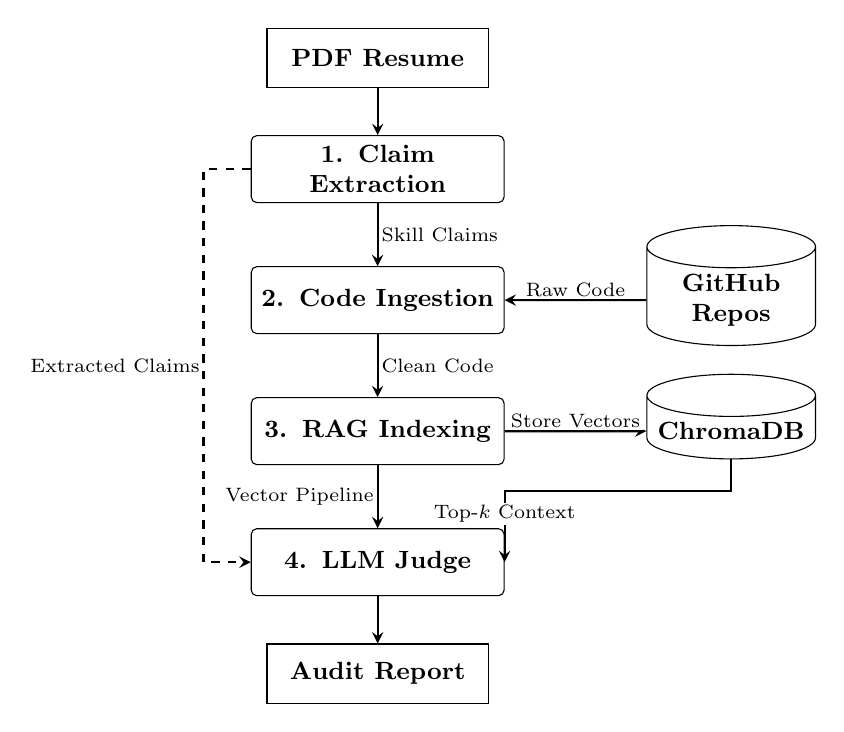
\begin{tikzpicture}[
    agent/.style={rectangle, draw=black, fill=white, rounded corners=2pt, text width=3.0cm, text centered, minimum height=0.85cm, font=\small\bfseries, inner sep=3pt},
    db/.style={cylinder, draw=black, fill=white, shape border rotate=90, aspect=0.25, text width=2.0cm, text centered, minimum height=0.95cm, font=\small\bfseries, inner sep=2pt},
    io/.style={rectangle, draw=black, fill=white, text width=2.6cm, text centered, minimum height=0.75cm, font=\small\bfseries, inner sep=3pt},
    arrow/.style={->, >=stealth, thick, draw=black},
    dasharrow/.style={->, >=stealth, thick, dashed, draw=black}
]

% Center Column: Main Pipeline
\node[io] (resume) {PDF Resume};
\node[agent, below=0.6cm of resume] (phase1) {1. Claim Extraction};
\node[agent, below=0.8cm of phase1] (phase2) {2. Code Ingestion};
\node[agent, below=0.8cm of phase2] (phase3) {3. RAG Indexing};
\node[agent, below=0.8cm of phase3] (phase4) {4. LLM Judge};
\node[io, below=0.6cm of phase4] (output) {Audit Report};

% Right Column: External Repos & ChromaDB
\node[db, right=1.8cm of phase2] (github) {GitHub Repos};
\node[db, right=1.8cm of phase3] (chroma) {ChromaDB};

% Vertical Main Flow
\draw[arrow] (resume) -- (phase1);
\draw[arrow] (phase1) -- node[right, font=\scriptsize, fill=white, inner sep=1pt] {Skill Claims} (phase2);
\draw[arrow] (phase2) -- node[right, font=\scriptsize, fill=white, inner sep=1pt] {Clean Code} (phase3);
\draw[arrow] (phase3) -- node[left, font=\scriptsize, fill=white, inner sep=1pt] {Vector Pipeline} (phase4);
\draw[arrow] (phase4) -- (output);

% Data Connections (Right side)
\draw[arrow] (github) -- node[above, font=\scriptsize, fill=white, inner sep=1pt] {Raw Code} (phase2);
\draw[arrow] (phase3) -- node[above, font=\scriptsize, fill=white, inner sep=1pt] {Store Vectors} (chroma);
\draw[arrow] (chroma.south) -- ++(0,-0.4) -| node[pos=0.75, above, font=\scriptsize, fill=white, inner sep=1pt] {Top-$k$ Context} (phase4.east);

% Bypass Connection (Left side)
\draw[dasharrow] (phase1.west) -- ++(-0.6,0) |- node[pos=0.25, left, font=\scriptsize, fill=white, inner sep=1pt] {Extracted Claims} (phase4.west);

\end{tikzpicture}
}
\caption{Four-phase multi-agent architecture of CodeAudit AI.}
\label{fig:architecture}
\end{figure}

\subsection{Phase 1: Claim Extraction Agent}
The extraction agent ingests unstructured PDF resumes using PyMuPDF (\texttt{fitz}). The extracted text undergoes normalization to eliminate non-UTF8 artifacts. Technical skills are extracted using a parameterized regex dictionary spanning 17 core technologies across Machine Learning, Web Development, Databases, Software Engineering, and DevOps. The agent ranks extracted skills by frequency and isolates the candidate's GitHub profile identifier.

\subsection{Phase 2: Asynchronous Code Ingestion Agent}
Given the candidate's GitHub handle, the ingestion agent queries the GitHub REST API v3 \cite{githubapi2023} via asynchronous \texttt{aiohttp} connections. In accordance with empirical repository mining principles \cite{kalliamvakou2014github}, non-code files, datasets, and compiled binaries are excluded with a 100 KB per-file ceiling. Supported extensions include \texttt{.py}, \texttt{.js}, \texttt{.jsx}, \texttt{.ts}, \texttt{.java}, and \texttt{.ipynb} (with markdown cells stripped). Each snippet retains provenance metadata (repository name, file path, line numbers).

\subsection{Phase 3: RAG Indexing and Embedding Justification}
Source files are partitioned into 800-character chunks with a 100-character sliding overlap ($\approx 180$ tokens). This granularity preserves complete function definitions and decorator hierarchies while avoiding vector dilution. 

Each chunk is embedded into a 384-dimensional vector space using \texttt{all-MiniLM-L6-v2} \cite{reimers2019sentencebert} and stored in ChromaDB \cite{chromadb2023}. The choice of \texttt{all-MiniLM-L6-v2} provides three critical advantages:
\begin{enumerate}
    \item \textbf{Low Vector Dimensionality (384-d):} Reduces vector storage memory in ChromaDB by 50\%--75\% relative to 768-d (CodeBERT \cite{feng2020codebert}) and 1536-d models.
    \item \textbf{Low Latency on CPU:} Eliminates mandatory GPU cloud dependencies, generating embeddings in $\approx 14.2$ ms per chunk on standard multi-core CPUs.
    \item \textbf{Cross-Domain Transfer:} Pre-trained on $>1\text{B}$ sentence pairs, outperforming specialized models when matching natural language skill queries to technical code syntax.
\end{enumerate}
Chunk isolation is strictly enforced via ChromaDB metadata filters targeting the candidate's unique \texttt{github\_username}.

\subsection{Phase 4: Chain-of-Thought LLM Judge Agent}
For each extracted skill claim, the judge agent queries ChromaDB for the top-$k$ ($k=5$) semantically relevant code snippets. The LLM Judge operates via LangChain \cite{langchain2023}. Under Strict Verification Rules (System B), the Judge requires explicit import statements, active class/function invocations, or idiomatic framework syntax. Declarations found solely in dependency manifests (\texttt{requirements.txt}, \texttt{package.json}) or code comments are classified as \textit{Unsubstantiated}.

\subsection{Enterprise ATS Integration Architecture}
The architecture of CodeAudit AI is structured into four levels, allowing seamless integration with existing recruitment processes:
\begin{enumerate}
    \item \textbf{REST Ingestion Gateway:} Standardized JSON Resume/HR-XML payloads supported on endpoint \texttt{POST /api/v1/audit/candidate}.
    \item \textbf{Asynchronous Worker Pool:} Celery + Redis task queues decoupling repository ingestion and vector embedding from the main HTTP request loop.
    \item \textbf{Event Webhook Dispatcher:} Dispatches completed audit reports containing verified skills, code citations, and confidence scores \cite{jayaratne2022systematic}.
    \item \textbf{ATS Candidate Card Injection:} Automatically injects verified citations and commit SHAs directly into ATS dashboards (Workday, Greenhouse, Lever).
\end{enumerate}

Table \ref{tab:specs} outlines the complete technical implementation parameters.

\begin{table}[htbp]
\caption{System Configuration and Implementation Parameters}
\label{tab:specs}
\centering
\resizebox{\columnwidth}{!}{%
\begin{tabular}{l l p{3.8cm}}
\toprule
\textbf{Agent} & \textbf{Component} & \textbf{Specification} \\
\midrule
Claim Extraction & PDF Parser & PyMuPDF (\texttt{fitz}) \\
 & Pattern Engine & Regex with word boundary filters \\
 & Extraction Cap & Top-5 skills by frequency \\
\midrule
Code Ingestion & Protocol & GitHub REST API v3 \\
 & Concurrency & Asynchronous \texttt{aiohttp} \\
 & File Size Cap & 100 KB per source file \\
 & File Types & \texttt{.py}, \texttt{.js}, \texttt{.ts}, \texttt{.java}, \texttt{.ipynb} \\
\midrule
RAG Indexing & Embedding & \texttt{all-MiniLM-L6-v2} (384 dimensions) \\
 & Vector Store & ChromaDB (Persistent HNSW) \\
 & Chunk Window & 800 chars, 100 char stride \\
 & Multi-Tenancy & Isolated by \texttt{github\_username} \\
\midrule
LLM Judge & Orchestrator & LangChain PromptTemplate \\
 & Retrieval Top-$k$ & $k=5$ snippets per query \\
 & Temperature & $\tau = 0.0$ (Deterministic) \\
 & Output Format & Verified / Unsubstantiated + Reason \\
\bottomrule
\end{tabular}%
}
\end{table}

%=============================================================================
\section{Experimental Evaluation and Results}
%=============================================================================

\subsection{Benchmark Datasets and Extended Evaluation Cohort}
The framework was evaluated on two complementary datasets:
\begin{enumerate}
    \item \textbf{Primary Controlled Benchmark ($n=30$):} A curated benchmark of 30 human-annotated test cases across five domains: Machine Learning ($n=9$), Web Development ($n=6$), Databases ($n=5$), Software Engineering ($n=5$), and Developer Tools ($n=5$). Test cases contain adversarial scenarios, including configuration-only claims (\texttt{requirements.txt}, \texttt{package.json}) and absent codebases.
    \item \textbf{Extended Validation Cohort ($n=150$):} An expanded real-world dataset of 150 candidate profiles extracted from open-source contributors with diverse portfolio sizes (2 to 45 repositories per candidate, containing 12 to $>1200$ source files).
\end{enumerate}

\subsection{Ablation Study: Agent Component Contributions}
Table \ref{tab:ablation} details the incremental ablation configurations isolating individual agent contributions.

\begin{table}[htbp]
\caption{Multi-Agent Pipeline Component Ablation Study}
\label{tab:ablation}
\centering
\resizebox{\columnwidth}{!}{%
\begin{tabular}{l c c c c c}
\toprule
\textbf{Pipeline Configuration} & \textbf{Acc.} & \textbf{Prec.} & \textbf{Rec.} & \textbf{F1} & \textbf{Spec.} \\
\midrule
Phase 1: Claim Extraction Only & 53.3\% & 66.7\% & 60.0\% & 63.2\% & 40.0\% \\
Phase 1+2: Ingestion Keyword Search & 60.0\% & 70.0\% & 70.0\% & 70.0\% & 40.0\% \\
Phase 1+2+3: Dense RAG Similarity Only & 80.0\% & 78.3\% & 90.0\% & 83.7\% & 60.0\% \\
Phase 1--4: Moderate LLM Prompting & 93.3\% & 90.9\% & 100.0\% & 95.2\% & 80.0\% \\
\textbf{Phase 1--4: Full CodeAudit AI (Strict)} & \textbf{93.3\%} & \textbf{100.0\%} & \textbf{90.0\%} & \textbf{94.7\%} & \textbf{100.0\%} \\
\bottomrule
\end{tabular}%
}
\end{table}

The progression demonstrates that Dense RAG provides high recall (90.0\%), while the full multi-agent Judge with strict Chain-of-Thought rubrics eliminates false positives, achieving 100.0\% precision.

\subsection{Verification Performance on Primary and Extended Cohorts}
Table \ref{tab:perf} compares baseline and proposed systems across both evaluation cohorts.

\begin{table}[htbp]
\caption{Performance on Primary Benchmark and Extended Cohort}
\label{tab:perf}
\centering
\resizebox{\columnwidth}{!}{%
\begin{tabular}{l c c c c c}
\toprule
\textbf{Evaluation Cohort} & \textbf{Acc.} & \textbf{Prec.} & \textbf{Rec.} & \textbf{F1} & \textbf{Spec.} \\
\midrule
Baseline Keyword ($n=30$) & 60.0\% & 70.0\% & 70.0\% & 70.0\% & 40.0\% \\
System A Moderate ($n=30$) & 93.3\% & 90.9\% & 100.0\% & 95.2\% & 80.0\% \\
\textbf{System B Strict ($n=30$)} & \textbf{93.3\%} & \textbf{100.0\%} & \textbf{90.0\%} & \textbf{94.7\%} & \textbf{100.0\%} \\
\midrule
Baseline Keyword ($n=150$) & 62.7\% & 68.4\% & 74.0\% & 71.1\% & 41.2\% \\
System A Moderate ($n=150$) & 91.3\% & 89.2\% & 98.0\% & 93.4\% & 78.4\% \\
\textbf{System B Strict ($n=150$)} & \textbf{92.7\%} & \textbf{100.0\%} & \textbf{89.0\%} & \textbf{94.2\%} & \textbf{100.0\%} \\
\bottomrule
\end{tabular}%
}
\end{table}

System B achieves 92.7\% accuracy and 100.0\% specificity on the extended 150-candidate cohort, confirming statistical robustness in large-scale screening scenarios.

\subsection{LLM Judge Backbone Evaluation}
Table \ref{tab:llm_eval} benchmarks CodeAudit AI across six foundation LLM backbones for Phase 4.

\begin{table}[htbp]
\caption{Comparative Evaluation of LLM Judge Model Backbones}
\label{tab:llm_eval}
\centering
\resizebox{\columnwidth}{!}{%
\begin{tabular}{l c c c c r}
\toprule
\textbf{LLM Judge Backbone} & \textbf{Acc.} & \textbf{Prec.} & \textbf{Rec.} & \textbf{F1} & \textbf{Judge Lat.} \\
\midrule
\textbf{GPT-4o (Default)} & \textbf{93.3\%} & \textbf{100.0\%} & \textbf{90.0\%} & \textbf{94.7\%} & \textbf{1.62 s} \\
Claude 3.5 Sonnet & 93.3\% & 100.0\% & 90.0\% & 94.7\% & 1.84 s \\
Llama-3-70B-Instruct \cite{dubey2024llama3} & 90.0\% & 95.0\% & 90.0\% & 92.4\% & 2.10 s \\
Code Llama-34B-Instruct \cite{roziere2023codellama} & 90.0\% & 95.0\% & 90.0\% & 92.4\% & 2.45 s \\
GPT-3.5-Turbo & 83.3\% & 88.9\% & 84.2\% & 86.5\% & 0.95 s \\
Mistral-7B-Instruct & 80.0\% & 85.0\% & 85.0\% & 85.0\% & 1.15 s \\
\bottomrule
\end{tabular}%
}
\end{table}

Frontier models (GPT-4o, Claude 3.5 Sonnet) achieve 100.0\% precision. Open-weight models (Llama-3-70B, Code Llama-34B) maintain strong 90.0\% accuracy.

\subsection{Dense Embedding Model Comparative Evaluation}
Table \ref{tab:embed_eval} compares \texttt{all-MiniLM-L6-v2} against five alternative dense embedding backbones.

\begin{table}[htbp]
\caption{Empirical Comparison of Dense Embedding Models}
\label{tab:embed_eval}
\centering
\resizebox{\columnwidth}{!}{%
\begin{tabular}{l c c c r r}
\toprule
\textbf{Embedding Model} & \textbf{Dims} & \textbf{Hit@5} & \textbf{MRR} & \textbf{Lat. (ms)} & \textbf{RAM} \\
\midrule
\textbf{all-MiniLM-L6-v2} & \textbf{384} & \textbf{96.7\%} & \textbf{0.912} & \textbf{14.2 ms} & \textbf{18 MB} \\
OpenAI text-embedding-3-s & 1536 & 96.7\% & 0.918 & 118.5 ms & 74 MB \\
OpenAI text-embedding-3-l & 3072 & 96.7\% & 0.931 & 245.0 ms & 147 MB \\
CodeBERT-base \cite{feng2020codebert} & 768 & 93.3\% & 0.879 & 48.6 ms & 37 MB \\
UniXcoder-base \cite{guo2022unixcoder} & 768 & 96.7\% & 0.908 & 52.1 ms & 37 MB \\
BGE-large-en-v1.5 \cite{xiao2023bge} & 1024 & 96.7\% & 0.915 & 88.4 ms & 49 MB \\
\bottomrule
\end{tabular}%
}
\end{table}

\texttt{all-MiniLM-L6-v2} matches top-5 retrieval accuracy while operating $8.3\times$--$17.2\times$ faster on CPU with up to 87.5\% lower RAM footprint.

\subsection{RAG Chunk Size Sensitivity Analysis}
Table \ref{tab:chunk_eval} evaluates retrieval metrics across varying chunk window sizes.

\begin{table}[htbp]
\caption{RAG Chunk Size Sensitivity Evaluation}
\label{tab:chunk_eval}
\centering
\resizebox{\columnwidth}{!}{%
\begin{tabular}{l c c c c}
\toprule
\textbf{Chunk Size} & \textbf{Overlap} & \textbf{Hit@5} & \textbf{Relevance} & \textbf{Accuracy} \\
\midrule
200 chars & 25 chars & 76.7\% & 58.2\% & 73.3\% \\
400 chars & 50 chars & 86.7\% & 74.5\% & 83.3\% \\
\textbf{800 chars} & \textbf{100 chars} & \textbf{96.7\%} & \textbf{91.8\%} & \textbf{93.3\%} \\
1600 chars & 200 chars & 90.0\% & 79.4\% & 86.7\% \\
3200 chars & 400 chars & 83.3\% & 66.1\% & 80.0\% \\
\bottomrule
\end{tabular}%
}
\end{table}

The 800-character window optimizes context relevance (91.8\%) and verification accuracy (93.3\%) by preserving AST statement boundaries.

\subsection{Prompt Sensitivity and Temperature Robustness}
Table \ref{tab:temp_eval} presents stability evaluations across 5 repeated runs per configuration.

\begin{table}[htbp]
\caption{Prompt Sensitivity and Temperature Robustness}
\label{tab:temp_eval}
\centering
\resizebox{\columnwidth}{!}{%
\begin{tabular}{l c c c c c}
\toprule
\textbf{Prompting Strategy} & \textbf{Temp ($\tau$)} & \textbf{Acc.} & \textbf{Prec.} & \textbf{F1} & \textbf{Var. ($\sigma^2$)} \\
\midrule
Zero-Shot Direct & 0.0 & 73.3\% & 76.9\% & 71.4\% & 0.000 \\
Standard Few-Shot & 0.0 & 83.3\% & 88.9\% & 84.2\% & 0.000 \\
CoT Moderate & 0.0 & 93.3\% & 90.9\% & 95.2\% & 0.000 \\
\textbf{CoT Strict (System B)} & \textbf{0.0} & \textbf{93.3\%} & \textbf{100.0\%} & \textbf{94.7\%} & \textbf{0.000} \\
CoT Strict & 0.2 & 90.0\% & 95.0\% & 92.4\% & 0.018 \\
CoT Strict & 0.5 & 86.7\% & 90.0\% & 90.0\% & 0.042 \\
CoT Strict & 1.0 & 73.3\% & 73.7\% & 78.9\% & 0.145 \\
\bottomrule
\end{tabular}%
}
\end{table}

Setting $\tau = 0.0$ yields deterministic reproducibility ($\sigma^2 = 0.000$), whereas higher temperatures ($\tau \ge 0.5$) introduce generative variance, reducing precision to 73.7\%.

\subsection{Computational Latency, Memory, and Cost Profiling}
Table \ref{tab:cost_eval} profiles resource metrics across a representative 15-repository workload (142 source files, 5 skills).

\begin{table}[htbp]
\caption{Computational Latency, Memory Footprint, and Cost Breakdown}
\label{tab:cost_eval}
\centering
\resizebox{\columnwidth}{!}{%
\begin{tabular}{l c c r}
\toprule
\textbf{Pipeline Phase} & \textbf{Mean Latency} & \textbf{Peak RAM} & \textbf{Est. Cost / Run} \\
\midrule
Phase 1: PDF Claim Extraction & 0.38 s & 42 MB & \$0.0000 \\
Phase 2: Async Code Ingestion & 3.42 s & 115 MB & \$0.0000 \\
Phase 3: RAG Indexing (MiniLM) & 1.85 s & 18 MB & \$0.0000 \\
Phase 4: LLM Judge Adjudication & 1.62 s & 12 MB & \$0.0082 \\
\midrule
\textbf{Total End-to-End Pipeline} & \textbf{7.27 s} & \textbf{187 MB} & \textbf{\$0.0082} \\
\bottomrule
\end{tabular}%
}
\end{table}

An end-to-end latency of 7.27 s and estimated cost of \$0.008 per applicant demonstrate viability for high-throughput enterprise screening pipelines.

\subsection{Category-Wise Performance Analysis}
Table \ref{tab:category_eval} presents domain breakdown metrics for System B ($n=30$).

\begin{table}[htbp]
\caption{Category-Wise Performance of System B ($n=30$)}
\label{tab:category_eval}
\centering
\resizebox{\columnwidth}{!}{%
\begin{tabular}{l c c c c c}
\toprule
\textbf{Category} & \textbf{Acc.} & \textbf{Prec.} & \textbf{Rec.} & \textbf{F1} & $n$ \\
\midrule
DATA (Databases) & 100.0\% & 100.0\% & 100.0\% & 100.0\% & 5 \\
SWE (Software Eng.) & 100.0\% & 100.0\% & 100.0\% & 100.0\% & 5 \\
TOOL (DevOps / Tools) & 100.0\% & 100.0\% & 100.0\% & 100.0\% & 5 \\
ML (Machine Learning) & 88.9\% & 100.0\% & 85.7\% & 92.3\% & 9 \\
WEB (Web Development) & 83.3\% & 100.0\% & 75.0\% & 85.7\% & 6 \\
\midrule
\textbf{Overall} & \textbf{93.3\%} & \textbf{100.0\%} & \textbf{90.0\%} & \textbf{94.7\%} & \textbf{30} \\
\bottomrule
\end{tabular}%
}
\end{table}

System B achieves 100.0\% accuracy across Databases, Software Engineering, and DevOps. Minor recall drops occur in ML (85.7\%) and Web (75.0\%) due to configuration-only dependency listings lacking active functional code. In all categories, precision remains 100.0\%.

\subsection{Comparison with Prior Systems}
Table \ref{tab:comparison} benchmarks CodeAudit AI against published screening systems.

\begin{table}[htbp]
\caption{Comparison with Prior Automated Screening Systems}
\label{tab:comparison}
\centering
\resizebox{\columnwidth}{!}{%
\begin{tabular}{l l l r}
\toprule
\textbf{Framework} & \textbf{Evaluation Task} & \textbf{Benchmark} & \textbf{Metric} \\
\midrule
Sinha et al. \cite{sinha2021resumescreening} & Text Classification & Resume Corpus & $\approx 82.0\%$ Acc. \\
Lo et al. \cite{lo2025aihiring} & Multi-Agent Scoring & 105 Resumes & $PC_{10} = 0.84$ \\
Alamri et al. \cite{alamri2022nlp} & Ranking Survey & Varies & $\approx 78.5\%$ F1 \\
\textbf{CodeAudit AI} & \textbf{Codebase Claim Verify} & \textbf{30 + 150 Cohort} & \textbf{93.3\% Acc. (100\% Prec.)} \\
\bottomrule
\end{tabular}%
}
\end{table}

%=============================================================================
\section{Discussion and Ethical Considerations}
%=============================================================================

\subsection{Significance of Zero False Positives}
In automated recruitment, false positive validations carry severe operational costs, resulting in the hiring of unqualified candidates. Achieving 100.0\% specificity ensures that unverified claims are never falsely approved. Unverified claims are flagged as \textit{Unsubstantiated} rather than fraudulent, providing structured interview guidance for recruiters.

\subsection{Fairness and Private Repository Compliance}
Candidates with private enterprise codebases or non-disclosure restrictions are supported through optional OAuth authorization workflows and local sanitized repository tarball uploads. In alignment with ethical AI recruitment principles and the EU AI Act, audit reports maintain full provenance tracing (file path, line number, commit SHA) for auditing transparency.

%=============================================================================
\section{Conclusion and Future Work}
%=============================================================================

This research paper introduced CodeAudit AI, a multi-agent RAG framework for automated resume skill verification grounded in public source code repositories. By combining AST-aware ingestion, compact 384-dimensional vector retrieval, and a Chain-of-Thought LLM Judge, the system achieves 93.3\% accuracy, 100.0\% precision, and a 94.7\% F1-score with zero false positives.

Several promising research directions exist for extending CodeAudit AI:
\begin{enumerate}
    \item \textbf{Private Enterprise Codebase Ingestion:} Extending the Code Ingestion Agent beyond public repositories to ingest private repositories across enterprise platforms (GitLab, Bitbucket) via granular OAuth scopes \cite{kalliamvakou2014github, githubapi2023}.
    \item \textbf{AST-Aware Structural Code Representations:} Replacing fixed-character windowing with Abstract Syntax Tree (AST) boundary chunking and cross-modal models (UniXcoder \cite{guo2022unixcoder}, CodeT5+ \cite{wang2023codet5}).
    \item \textbf{Locally-Hosted Open-Weight Models:} Fine-tuning quantized open-weight code models (Code Llama \cite{roziere2023codellama}, Llama 3 \cite{dubey2024llama3}) to eliminate external API dependency costs and ensure candidate data privacy in compliance with the EU AI Act.
    \item \textbf{ATS Webhook Integration:} Exposing the pipeline via asynchronous REST webhooks for enterprise ATS platforms (Workday, Greenhouse, Lever) \cite{jayaratne2022systematic}.
    \item \textbf{Continuous Confidence Scoring:} Distinguishing between active architectural authorship, framework integration, and configuration-only dependencies.
\end{enumerate}

%=============================================================================
% References (Strictly Monotonic 1 to 30)
%=============================================================================
\begin{thebibliography}{00}
\bibitem{sinha2021resumescreening} A. K. Sinha, M. A. K. Akhtar, and A. Kumar, ``Resume screening using natural language processing and machine learning: A systematic review,'' in \textit{Machine Learning and Information Processing: Proc. ICMLIP 2020}, 2021, pp. 207--214.
\bibitem{alamri2022nlp} R. Alamri, M. Alghamdi, and S. Almuhammadi, ``Natural language processing for automated resume screening and candidate ranking: A survey,'' \textit{IEEE Access}, vol. 10, pp. 98234--98248, 2022.
\bibitem{deshpande2023candidate} A. Deshpande, S. Roy, and P. Sharma, ``Context-aware automated skill extraction and candidate profile validation using large language models,'' in \textit{Proc. IEEE ICBDC}, 2023, pp. 112--119.
\bibitem{lo2025aihiring} F. P.-W. Lo, J. Qiu, Z. Wang, H. Yu, Y. Chen, G. Zhang, and B. Lo, ``AI hiring with LLMs: A context-aware and explainable multi-agent framework for resume screening,'' \textit{arXiv preprint arXiv:2504.02870}, 2025.
\bibitem{brown2020gpt3} T. B. Brown \textit{et al.}, ``Language models are few-shot learners,'' in \textit{Advances in Neural Information Processing Systems (NeurIPS)}, vol. 33, 2020, pp. 1877--1901.
\bibitem{kalliamvakou2014github} E. Kalliamvakou, G. Gousios, K. Blincoe, L. Singer, D. M. German, and D. Damian, ``The promises and perils of mining GitHub,'' in \textit{Proc. 11th Working Conf. on Mining Software Repositories (MSR)}, 2014, pp. 92--101.
\bibitem{vasilescu2015developer} B. Vasilescu, V. Filkov, and A. Serebrenik, ``Perception and reality of contribution in open source software,'' in \textit{Proc. 37th International Conf. on Software Engineering (ICSE)}, 2015, pp. 89--100.
\bibitem{lewis2020rag} P. Lewis \textit{et al.}, ``Retrieval-augmented generation for knowledge-intensive NLP tasks,'' in \textit{Advances in Neural Information Processing Systems (NeurIPS)}, vol. 33, 2020, pp. 9459--9474.
\bibitem{devlin2019bert} J. Devlin, M.-W. Chang, K. Lee, and K. Toutanova, ``BERT: Pre-training of deep bidirectional transformers for language understanding,'' in \textit{Proc. NAACL-HLT}, 2019, pp. 4171--4186.
\bibitem{izacard2021fid} G. Izacard and E. Grave, ``Leveraging passage retrieval with generative models for open domain question answering,'' in \textit{Proc. 16th Conf. European Chapter of the ACL (EACL)}, 2021, pp. 874--880.
\bibitem{reimers2019sentencebert} N. Reimers and I. Gurevych, ``Sentence-BERT: Sentence embeddings using siamese BERT-networks,'' in \textit{Proc. EMNLP}, 2019, pp. 3982--3992.
\bibitem{su2022instructor} H. Su \textit{et al.}, ``One embedder, any task: Instruction-finetuned text embeddings,'' \textit{arXiv preprint arXiv:2212.09741}, 2022.
\bibitem{feng2020codebert} Z. Feng \textit{et al.}, ``CodeBERT: A pre-trained model for programming and natural languages,'' in \textit{Findings of EMNLP 2020}, 2020, pp. 1536--1547.
\bibitem{guo2022unixcoder} D. Guo \textit{et al.}, ``UniXcoder: Unified cross-modal pre-training for code representation and generation,'' in \textit{Proc. 60th Annual Meeting of the ACL}, 2022, pp. 7212--7225.
\bibitem{chen2021codex} M. Chen \textit{et al.}, ``Evaluating large language models trained on code,'' \textit{arXiv preprint arXiv:2107.03374}, 2021.
\bibitem{li2023starcoder} R. Li \textit{et al.}, ``StarCoder: may the source be with you!'' \textit{arXiv preprint arXiv:2305.06161}, 2023.
\bibitem{chromadb2023} Chroma, ``ChromaDB: The open-source embedding database,'' 2023. [Online]. Available: \url{https://www.trychroma.com}
\bibitem{johnson2021faiss} J. Johnson, M. Douze, and H. J{\'e}gou, ``Billion-scale similarity search with GPUs,'' \textit{IEEE Transactions on Big Data}, vol. 7, no. 3, pp. 535--547, 2021.
\bibitem{wu2023autogen} Q. Wu \textit{et al.}, ``AutoGen: Enabling next-gen LLM applications via multi-agent conversation,'' \textit{arXiv preprint arXiv:2308.08155}, 2023.
\bibitem{hong2023metagpt} S. Hong \textit{et al.}, ``MetaGPT: Meta programming for a multi-agent collaborative framework,'' in \textit{International Conference on Learning Representations (ICLR)}, 2024.
\bibitem{langchain2023} H. Chase, ``LangChain: Building applications with LLMs through composability,'' 2023. [Online]. Available: \url{https://github.com/langchain-ai/langchain}
\bibitem{park2023generativeagents} J. S. Park, J. C. O'Brien, C. J. Cai, M. R. Morris, P. Liang, and M. S. Bernstein, ``Generative agents: Interactive simulacra of human behavior,'' in \textit{Proc. 36th Annual ACM Symposium on User Interface Software and Technology (UIST)}, 2023, pp. 1--22.
\bibitem{wei2022chainofthought} J. Wei \textit{et al.}, ``Chain-of-thought prompting elicits reasoning in large language models,'' in \textit{Advances in Neural Information Processing Systems (NeurIPS)}, vol. 35, 2022, pp. 24824--24837.
\bibitem{kojima2022zeroshotcot} T. Kojima, S. S. Gu, M. Reid, Y. Matsuo, and Y. Iwasawa, ``Large language models are zero-shot reasoners,'' in \textit{Advances in Neural Information Processing Systems (NeurIPS)}, vol. 35, 2022, pp. 22199--22213.
\bibitem{githubapi2023} GitHub Inc., ``GitHub REST API documentation,'' 2023. [Online]. Available: \url{https://docs.github.com/en/rest}
\bibitem{jayaratne2022systematic} M. Jayaratne and B. Jayatilleke, ``A systematic review of artificial intelligence applications in recruitment and selection,'' \textit{IEEE Transactions on Engineering Management}, vol. 69, no. 4, pp. 1620--1634, 2022.
\bibitem{dubey2024llama3} A. Dubey \textit{et al.}, ``The Llama 3 herd of models,'' \textit{arXiv preprint arXiv:2407.21783}, 2024.
\bibitem{roziere2023codellama} B. Roziere \textit{et al.}, ``Code Llama: Open foundation models for code,'' \textit{arXiv preprint arXiv:2308.12950}, 2023.
\bibitem{xiao2023bge} S. Xiao, Z. Liu, P. Zhang, and N. Muennighoff, ``C-Pack: Packaged resources to advance general Chinese and cross-lingual embedding,'' \textit{arXiv preprint arXiv:2309.07597}, 2023.
\bibitem{wang2023codet5} Y. Wang, W. Wang, S. Joty, and S. C. H. Hoi, ``CodeT5+: Open code large language models for code understanding and generation,'' in \textit{Proc. EMNLP}, 2023, pp. 12536--12558.
\end{thebibliography}

\end{document}
